\section{Εφαρμογή με 2 σένσορες και έναν ενεργοποιητή}
\label{sec:example1}

Σε αυτό το παράδειγμα αναλύεται η χρήση των παραπάνω εργαλείων για την ανάπτυξη μιας εφαρμογής για τη λήψη διαφόρων μετρήσεων από περιφερειακά. Το σύστημα αποτελείται από έναν μικροελεγκτή NodeMCU ESP32 που αποτελεί την κύρια υπολογιστική μονάδα, ένα σόναρ, έναν αισθητήρα περιβάλλοντος και έναν ενεργοποιητή με LED. Επίσης, χρησιμοποιείται και ένα raspberry pi στο οποίο τρέχει ένας broker. Οι συνδέσεις μεταξύ των συσκευών ορίστηκαν σε ένα αρχείο, χρησιμοποιώντας τη γλώσσα που αναλύεται στην \autoref{subsec:syntax_connections}. Το αρχείο για την περιγραφή των συνδέσεων που χρησιμοποιήθηκε είναι το ακόλουθο.

\newpage

\begin{lstlisting}
include srf04
include bme680
include ws281x
include esp32_wroom_32

connection:
	name: sonar_esp32
	board: esp32_wroom_32
	peripheral: srf04
	power_connections:
		- gnd_1 -- gnd
		- power_5v -- vcc 
	hw_connections:
		- gpio: p_14 -- echo
		- gpio: p_13 -- trigger
	communication_endpoint:
		topic: srf04.data
		wifi_ssid: Wifi_2.4GHz
		wifi_passwd: okodikos?
		address: 2a02:587:541f:44b6:a15:779:2a6e:f525
		port: 1885
		msg: Distance
		frequency: 5 hz

connection:
	name: bme680_esp32
	board: esp32_wroom_32
	peripheral: bme680
	power_connections:
		- gnd_1 -- gnd
		- power_5v -- vcc 
	hw_connections:
		- i2c: 
			sda: p_21 -- sda
			scl: p_22 -- scl
			slave_address: 0x76
	communication_endpoint:
		topic: bme680.data
		wifi_ssid: Wifi_2.4GHz
		wifi_passwd: okodikos?
		address: 2a02:587:541f:44b6:a15:779:2a6e:f525
		port: 1885
		msg: Env
		frequency: 2 hz

connection:
	name: ws281x_esp32
	board: esp32_wroom_32
	peripheral: ws281x
	power_connections:
		- gnd_1 -- gnd
		- power_5v -- vcc 
	hw_connections:
		- gpio: p_0 -- data_in
	communication_endpoint:
		topic: ws281x.data
		wifi_ssid: Wifi_2.4GHz
		wifi_passwd: okodikos?
		address: 2a02:587:541f:44b6:a15:779:2a6e:f525
		port: 1885
		msg: Leds_Controller
\end{lstlisting}

Για την παραγωγή του κώδικα εκτελέστηκε η παρακάτω εντολή.

\begin{lstlisting}
$ ./parser.py example1
\end{lstlisting}

Όπου example1 είναι το όνομα του παραπάνω αρχείου. Με την εκτέλεση της εντολής αυτής, παράγεται ένα αρχείο κώδικα C, ένα Makefile, μία εικόνα όπου φαίνεται η συνδεσμολογία των συσκευών και μια εικόνα όπου φαίνονται όλα τα χαρακτηριστικά του μοντέλου των συνδέσεων.. Τα αρχεία δημιουργήθηκαν σύμφωνα με τα πρότυπα αρχεία που παρουσιάζονται στο \autoref{appendix:templates}.

Στο \autoref{fig:example_connections} απεικονίζεται η συνδεσμολογία. Η δεύτερη εικόνα που παράχθηκε παρουσιάζεται στο \autoref{appendix:diagrams}.

\begin{figure}[!ht]
	\centering
	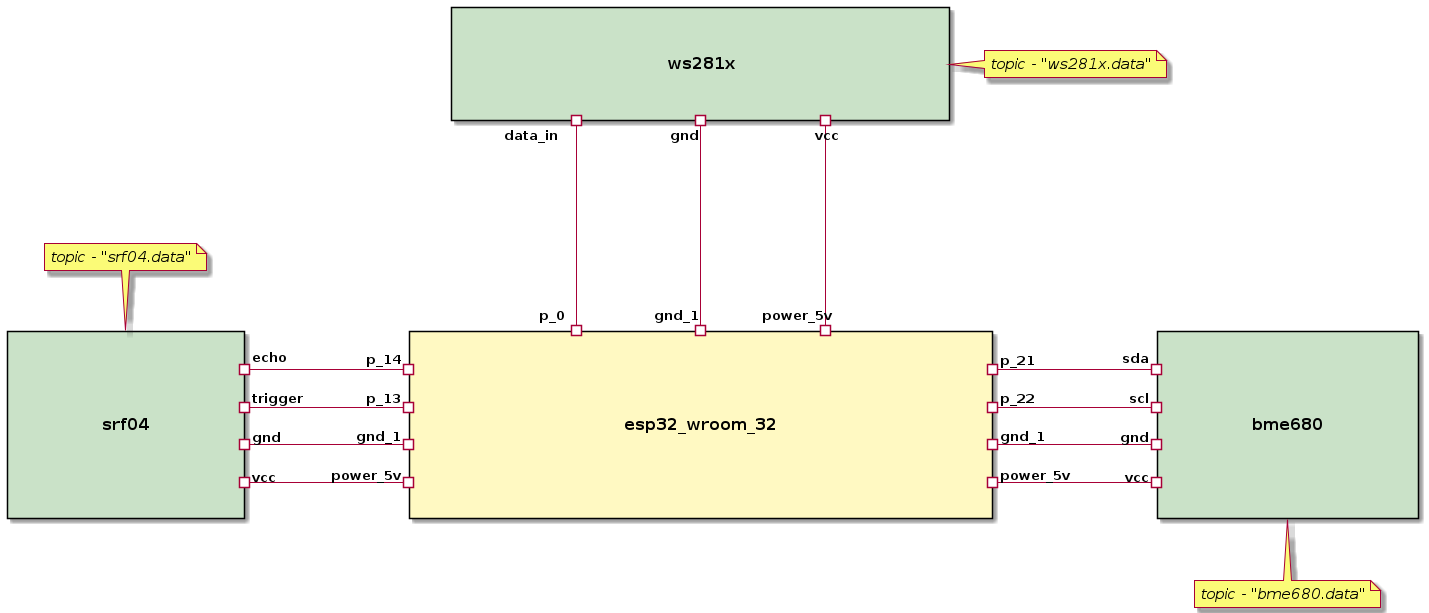
\includegraphics[width=1.0\textwidth]{./images/chapter6/example1a.png}
	\caption[\textit{Συνδεσμολογία μεταξύ των συσκευών}.]{\textit{Συνδεσμολογία μεταξύ των συσκευών}.}
	\label{fig:example_connections}
\end{figure}

Με την εκτέλεση των παραχθέντων αρχείων ξεκινάει ο έλεγχος των περιφερειακών. Υπάρχουν τα ακόλουθα τερματικά:

\begin{itemize}
	\item srf04.data: Εδώ κοινοποιούνται οι μετρήσεις από το sonar (απόσταση)
	\item bme680.data: Εδώ κοινοποιούνται οι μετρήσεις από τον αισθητήρα περιβάλλοντος (θερμοκρασία, υγρασία, πίεση)
	\item ws281x.data: Εδώ μπορούν να κοινοποιηθούν τιμές RGB, τις οποίες λαμβάνει ο ενεργοποιητής με τα LED και άρα τα ανάβει σύμφωνα με το δοσμένο χρώμα
\end{itemize}
